\documentclass[preprint,12pt]{elsarticle}

\usepackage{amssymb}
\usepackage[normalem]{ulem} % for \sout
\usepackage{xspace}

\journal{Science of Computer Programming}

\usepackage{hyperref}
\usepackage{color}

\newcommand{\definition}[1]{ 
\begin{quote} \item {\em #1} \end{quote}}
\newcommand {\chaptersummary}[1] { \vspace{3cm} \hrule \vspace{0.5cm} {\em #1 } \vspace{0.5cm} \hrule \vspace{0.5cm} \newpage}
\newcommand{\challenge}[1]{\paragraph {\bf \em [Challenge]} {\em #1}} 



\newcommand{\chapquote}[1]{\em #1} 


\newcommand{\quest}[1]{{\em ({\bf Mircea:} #1)}}
\newcommand{\mir}[1]{{\em ({\bf Mircea:} #1)}}
\newcommand{\mircea}[1]{{\em ({\bf Mircea:} #1)}}
\newcommand{\Mircea}[1]{{\em ({\bf Mircea:} #1)}}

\newcommand{\pg}[2]{#1 #2}
%\newcommand{\pg}[2]{\paragraph {#1} {\small #2}}
\newcommand{\mic}[1]{{\small #1}}

\definecolor{lg}{rgb}{0.9,0.9,0.9}
\definecolor{darkblue}{rgb}{0.0,0.0,0.5}


\newcommand{\cbar}{\vspace {1cm} \hrule }

\newcommand{\concls}[1]{\titlebox{Facts and Limitations}{#1}}

\newcommand{\titlebox}[2]{
\vspace{1cm}
\hrule
\vspace{0.25cm}
{\bf #1: }
\vspace{0.25cm}
\hrule
#2
\vspace{0.5cm}
}


% Utils

\newcommand{\dpdef}[1]{\paragraph{Definition.} {\em #1}}
\newcommand{\dpdisc}[1]{\paragraph {Discussion.} #1}
\newcommand{\dpr}[1]{\paragraph {Rationale.} #1}
\newcommand{\dpcat}[1]{\paragraph {Category:} #1}
\newcommand{\dpcatage}{\dpcat{Age-related}}
\newcommand{\dpcatdyn}{\dpcat{Dynamics-related}}
\newcommand{\dpexample}[1]{\paragraph {Example.} #1}
\newcommand{\dpp}[1]{\newpage\subsection{#1}}


\newcommand{\pidea}[1]{#1.}
\newcommand{\pideap}[1]{#1}
%\newcommand{\pidea}[1]{\paragraph{#1.}}
%\newcommand{\pideap}[1]{\paragraph{#1} }



\newcommand{\flabel}[1]{\label{fig:#1}}
\newcommand{\tlabel}[1]{\label{tab:#1}}
\newcommand{\clabel}[1]{\label{c:#1}}
\newcommand{\slab}[1]{\label{sec:#1}}

\newcommand{\fref}[1]{Figure \ref{fig:#1}}
\newcommand{\tref}[1]{Table \ref{tab:#1}}
\newcommand{\sref}[1]{Section \ref{sec:#1}}
\newcommand{\cref}[1]{Section \ref{c:#1}}

% Font conventions
\newcommand{\partref}[2]{{\bf Part \ref{p:#1}: #2}}
\newcommand{\chap}[1]{\item {\bf Chapter \ref{c:#1}} {\footnotesize (p.\pageref{c:#1})}}
\newcommand{\apdx}[1]{\item {\bf Appendix \ref{c:#1}} {\footnotesize (p.\pageref{c:#1})}}
\newcommand{\spref}[1]{Section \ref{sec:#1} {\footnotesize (p.\pageref{sec:#1})}}

\newcommand{\SOC}{\subsubsection* {Structure of the Chapter}}

\newcommand{\q}[1]{``#1''}

\newcommand{\tool}[1]{{\em #1}}
\newcommand{\pnam}[1]{{\em #1}}
\newcommand{\trm}[1]{{\em #1}}

\newcommand{\art}[1]{{\em #1}}
\newcommand{\book}[1]{{\em #1}}
\newcommand{\cit}[1]{{\em ``#1''}}

\newcommand{\proj}[1]{{\em #1}}
\newcommand{\dev}[1]{{\em #1}}
\newcommand{\term}[1]{{\em #1}}
\newcommand{\class}[1]{{\em #1}}
\newcommand{\method}[1]{{\em #1}}
\newcommand{\met}[1]{{\em #1}}
\newcommand{\pack}[1]{{\em #1}}
\newcommand{\model}[1]{{\em #1}}
\newcommand{\vp}[1]{{\em #1}}

\newcommand{\metric}[1]{{\em #1}}

\newcommand{\cod}[1]{{\em #1}}



% Tables with metrics
\newcommand{\metrictableh}[4]{
\begin{table}[h!]
%\footnotesize
\centering
\begin{tabular}{l l}
#1
\hline
#2
\hline
\end{tabular}
\caption{#3}\tlabel{#4}
\end{table}
}

\newcommand{\metrictable}[3]{
\metrictableh
{Acronym & Name\\}{#1}{#2}{#3}
}




% viewpoint definitions
\newcommand{\vpc}{black}
\newcommand{\Goal}[1]{\subsubsection* {Goal} #1}
\newcommand{\Cat}[1]{\subsubsection* {Category} #1}

\newcommand{\Concerns}[1]{\paragraph{\textcolor{\vpc}{Concerns}} \begin{itemize}#1\end{itemize}}
\newcommand{\Stakeholders}[1]{\paragraph{\textcolor{\vpc}{Stakeholders: }} #1}
\newcommand{\Construction}[1]{\subsubsection* {Construction Principles } #1}
\newcommand{\Navigation}[1]{\paragraph{\textcolor{\vpc}{Implementation in SPO.}}  #1}
\newcommand{\Examples}{\subsubsection{\textcolor{\vpc}{Examples}}}
\newcommand{\Discussion}[1]{\subsubsection{\textcolor{\vpc}{Discussion}} 
\begin{description}
#1
\end{description}}
\newcommand{\dpoint}[1]{\item {\em #1.} }
\newcommand{\cpoint}[1]{\item {\bf #1.} }
\newcommand{\cpointnp}[1]{\item {\bf #1} }



% Frequently Used Terms
% ---------------------

\newcommand{\Revenge}{{Revenge}\xspace}
\newcommand{\revenge}{{revenge}\xspace}
\renewcommand{\v}{viewpoint\xspace}

% Generic 
\newcommand{\ie}{\textit{i.e.,}\xspace}
\newcommand{\eg}{\textit{e.g.,}\xspace}
\newcommand{\etc}{\textit{etc.}\xspace}
\newcommand{\etal}{\textit{et al.}\xspace}


% Super-repositories / Ecosystems
\newcommand{\super}{super-repository\xspace}
\newcommand{\Super}{Super-Repository\xspace}
\newcommand{\Supers}{Super-Repositories\xspace}
\newcommand{\supers}{super-repositories\xspace}
\newcommand{\spo}{Small Project Observatory\xspace}
\newcommand{\tspo}{The Small Project Observatory\xspace}
\newcommand{\snaut}{Softwarenaut\xspace}
\newcommand{\store}{Store\xspace}
\newcommand{\svn}{SVN\xspace}
\newcommand{\LEM}{{Lightweight Ecosystem Model}\xspace}
\newcommand{\emlem}{{\em lightweight ecosystem model}\xspace}
\newcommand{\lem}{{lightweight ecosystem model}\xspace}
\newcommand{\emdpm}{{\em detailed project model}\xspace}
\newcommand{\dpm}{{detailed project model}\xspace}
\newcommand{\DPM}{{Detailed Project Model}\xspace}

\newcommand{\treveale}{the REVEAL ecosystem \xspace}
\newcommand{\reveal}{{REVEAL}\xspace}
\newcommand{\scg}{{SCG}\xspace}
\newcommand{\cincom}{{Cincom}\xspace}
\newcommand{\soops}{{Soops}\xspace}
\newcommand{\gnome}{{Gnome}\xspace}


%~~~~~~~~~~
%Viewpoints 
%~~~~~~~~~~
 \newcommand{\growth}{{Size Evolution}\xspace}
 \newcommand{\vgrowth}{{Size Evolution}\xspace}
 \newcommand{\vgrowthv}{{Size Evolution} viewpoint\xspace}

 \newcommand{\vacti}{{Activity Evolution}\xspace}
 \newcommand{\vactiv}{{Activity Evolution} viewpoint\xspace}

 \newcommand{\vcol}{{Developer Collaboration}\xspace}
 \newcommand{\vcolv}{{Developer Collaboration} viewpoint\xspace}

 \newcommand{\varch}{{Project Architecture}\xspace}
 \newcommand{\varchv}{{Project Architecture} viewpoint\xspace}

 \newcommand{\vtimeline}{{Developer Timelines}\xspace}
 \newcommand{\vtimelinev}{{Developer Timelines} viewpoint\xspace}

 \newcommand{\vpdep}{{Project Dependency Map}\xspace}
 \newcommand{\vpdepv}{{Project Dependency Map} viewpoint\xspace}

 \newcommand{\vpmat}{{Project Dependency Matrix}\xspace}
 \newcommand{\vpmatv}{{Project Dependency Matrix} viewpoint\xspace}



%~~~~~~~~~~~~~~
% Soops report
%~~~~~~~~~~~~~~

\newcommand{\soopsPart}[1]{\subsubsection* {\em #1}}





%
\newcommand{\s}{Softwarenaut\xspace}
\newcommand{\shrimp}{SHriMP\xspace}

% Package Patterns 
\newcommand{\Autonomous}{Autonomous\xspace}
\newcommand{\FallThrough}{Fall-Through\xspace}
\newcommand{\Iceberg}{Iceberg\xspace}
\newcommand{\Archipelago}{Archipelago\xspace}
\newcommand{\vpsem}{{\em vertical package slices}\xspace}
\newcommand{\vps}{vertical package slices\xspace}
\newcommand{\Vps}{Vertical package slices\xspace}
\newcommand{\VPS}{Vertical Package Slices\xspace}
\newcommand{\VPSem}{{\em Vertical Package Slices}\xspace}

% Dependency Evolution Patterns
\newcommand{\sdm}{{\em Semantic Dependency Matrix}\xspace}
\newcommand{\refil}{Relationship Evolution Filmstrip\xspace}




% -----------------------------------------------

\hypersetup{
    bookmarks=true,         % show bookmarks bar?
    unicode=false,          % non-Latin characters in Acrobat’s bookmarks
    pdftoolbar=true,        % show Acrobat’s toolbar?
    pdfmenubar=true,        % show Acrobat’s menu?
    pdffitwindow=false,     % window fit to page when opened
    pdfstartview={FitH},    % fits the width of the page to the window
    pdftitle={Reverse Engineering Software Ecosystems},    % title
    pdfauthor={Mircea Lungu},     		% author
    pdfsubject={Doctoral Dissertation},   	% subject of the document
    pdfcreator={Mircea Lungu},   		% creator of the document
    pdfproducer={Mircea Lungu}, 		% producer of the document
    pdfkeywords={keywords}, 			% list of keywords
    pdfnewwindow=true,      			% links in new window
    colorlinks=true,       			% false: boxed links; 
    linkcolor=darkblue,          		% color of internal links
    citecolor=darkblue,        			% color of links to bibliography
    filecolor=magenta,      			% color of file links
    urlcolor=cyan           			% color of external links
}




\graphicspath{{images/}}

\newcommand{\cd}[1]{{\em{#1}}}
%\newcommand{\ra}{$\rightarrow$}
%\newcommand{\chg}[2]{\textcolor{red}{\sout{#1}}{\ra}\textcolor{blue}{\uline{#2}}} % please change
%\newcommand{\ins}[1]{\textcolor{blue}{\uline{#1}}} % please insert
\newcommand{\rewritten}{\textcolor{red}{\uline{Rewritten}\ra\space }} % please insert

% ============================================================
% Markup macros for proof-reading
\usepackage{ifthen}
\usepackage[normalem]{ulem} % for \sout
\usepackage{xcolor}
\newcommand{\ra}{$\rightarrow$}
\newboolean{showedits}
\setboolean{showedits}{true} % toggle to show or hide edits
\ifthenelse{\boolean{showedits}}
{
	\newcommand{\ugh}[1]{\textcolor{red}{\uwave{#1}}} % please rephrase
	\newcommand{\ins}[1]{\textcolor{blue}{\uline{#1}}} % please insert
	\newcommand{\del}[1]{\textcolor{red}{\sout{#1}}} % please delete
	\newcommand{\chg}[2]{\textcolor{red}{\sout{#1}}{\ra}\textcolor{blue}{\uline{#2}}} % please change
}{
	\newcommand{\ugh}[1]{#1} % please rephrase
	\newcommand{\ins}[1]{#1} % please insert
	\newcommand{\del}[1]{} % please delete
	\newcommand{\chg}[2]{#2}
}
% ============================================================
% Put edit comments in a really ugly standout display
%\usepackage{ifthen}
\usepackage{amssymb}
\newboolean{showcomments}
\setboolean{showcomments}{true}
%\setboolean{showcomments}{false}
\newcommand{\id}[1]{$-$Id: scgPaper.tex 32478 2010-04-29 09:11:32Z oscar $-$}
\newcommand{\yellowbox}[1]{\fcolorbox{gray}{yellow}{\bfseries\sffamily\scriptsize#1}}
\newcommand{\triangles}[1]{{\sf\small$\blacktriangleright$\textit{#1}$\blacktriangleleft$}}
\ifthenelse{\boolean{showcomments}}
%{\newcommand{\nb}[2]{{\yellowbox{#1}\triangles{#2}}}
{\newcommand{\nbc}[3]{
 {\colorbox{#3}{\bfseries\sffamily\scriptsize\textcolor{white}{#1}}}
 {\textcolor{#3}{\sf\small$\blacktriangleright$\textit{#2}$\blacktriangleleft$}}}
 \newcommand{\version}{\emph{\scriptsize\id}}}
{\newcommand{\nbc}[3]{}
 \renewcommand{\ugh}[1]{#1} % please rephrase
 \renewcommand{\ins}[1]{#1} % please insert
 \renewcommand{\del}[1]{} % please delete
 \renewcommand{\chg}[2]{#2} % please change
 \newcommand{\version}{}}
\newcommand{\nb}[2]{\nbc{#1}{#2}{orange}}
\newcommand{\here}{\yellowbox{$\Rightarrow$ CONTINUE HERE $\Leftarrow$}}
\newcommand\rev[2]{\nb{TODO (rev #1)}{#2}} % reviewer comments
\newcommand\fix[1]{\nb{FIX}{#1}}
\newcommand\todo[1]{\nb{TO DO}{#1}}
\newcommand\on[1]{\nbc{ON}{#1}{red}} % add more author macros here
%\newcommand\XXX[1]{\nbc{XXX}{#1}{blue}}
%\newcommand\XXX[1]{\nbc{XXX}{#1}{brown}}
%\newcommand\XXX[1]{\nbc{XXX}{#1}{cyan}}
%\newcommand\XXX[1]{\nbc{XXX}{#1}{darkgray}}
%\newcommand\XXX[1]{\nbc{XXX}{#1}{gray}}
%\newcommand\XXX[1]{\nbc{XXX}{#1}{magenta}}
%\newcommand\XXX[1]{\nbc{XXX}{#1}{olive}}
%\newcommand\XXX[1]{\nbc{XXX}{#1}{orange}}
%\newcommand\XXX[1]{\nbc{XXX}{#1}{purple}}
%\newcommand\XXX[1]{\nbc{XXX}{#1}{red}}
%\newcommand\XXX[1]{\nbc{XXX}{#1}{teal}}
%\newcommand\XXX[1]{\nbc{XXX}{#1}{violet}}
% ============================================================
%\newcommand{\ie}{\emph{i.e.},\xspace}
\newcommand{\eg}{\emph{e.g.},\xspace}
\newcommand{\etal}{\emph{et al.}\xspace}
% ============================================================


\begin{document}

\begin{frontmatter}

%% Title, authors and addresses

\title{Evolutionary and Collaborative Software Architecture Recovery with Softwarenaut}
%\title{Softwarenaut: A Tool for Architecture Recovery }

\author{Mircea Lungu}
\address{Software Composition Group - University of Bern, Switzerland}

\author{Michele Lanza}
\address{REVEAL @ Faculty of Informatics - University of Lugano, Switzerland}

\author{Oscar Nierstrasz}
\address{Software Composition Group - University of Bern, Switzerland}

%%% abstract %%%

\begin{abstract}

Architecture recovery is an activity applied to a system whose initial architecture has eroded.
% \ugh{When the initial architecture of a system has eroded the only solution is architecture recovery.}
However, when the system under analysis is large, the user must use dedicated tools to support the recovery process. 

We present Softwarenaut -- a tool which supports architecture recovery through interactive exploration, evolutionary analysis and visualization.
\on{Missing one startling sentence}
It provides high-level and detailed perspectives which support the architecture recovery process as well as navigation primitives and filtering mechanisms that allow the complexity of large software systems to be managed.
% It provides \ugh{overview} and detailed perspectives which support the architecture recovery process as well as navigation primitives and filtering mechanisms that \ugh{allow managing} the complexity of large software systems.
The recovered architectural views can be shared between users through a Global Architectural View Repository thus allowing collaborative architecture recovery.
\on{What is cool or unusual? What will the reader learn? What is the key insight?!}

\end{abstract}

\begin{keyword}
Architecture Recovery \sep Visualization \sep Reverse Engineering
\end{keyword}

\end{frontmatter}

%%%%%%%%%%%%%%%%%%%%%%%%%%
\section{Introduction} \label{sec:Introduction}
%%%%%%%%%%%%%%%%%%%%%%

Any software system exists and functions within an environment; when this environment changes the system must change too or become obsolete \cite{lehman-softev}. As a result, maintaining a software system implies a continuous effort to keep it up to date with unanticipated changes in its environment. Having a clear and up to date understanding of the architecture of a system is critical for its maintenance and evolution \cite{Duca09c, pollet-sar}.

As a system evolves, its architecture erodes \cite{perry-foundations}: an architectural mismatch arises between the {\em as-defined} and {\em as-is} architecture \cite{garlan-mismatch}. One accompanying property of this continuous drift between the actual and the defined architecture of the system is an increasing brittleness of the system \cite{perry-foundations}. 

The main reason for architectural erosion and drift is widespread lack of programming language support for expressing the architecture, as well as the lack of tools that associate architectural decisions with the source code. The problem is an instance of the documentation problem: it is well known that the documentation of the system becomes quickly obsolete unless developers dedicate conscientious effort towards keeping it up to date \cite{riva-report}.

When the drift and erosion have brought the system architecture too far from the initial state, the solution is to recover the architecture of the system from the source code. Jazayeri defined architecture recovery as ``{\em the techniques and processes used to uncover a system's architecture from available information}'' \cite{jaza-archevo}. 

In the case of large software systems the architecture is specified through multiple architectural views that correspond to a set of given {\em architectural viewpoints}. An architectural viewpoint is a pattern or template from which to develop individual views by establishing the purposes and audience for a view and the techniques for its creation and analysis. Even if different authors propose different viewpoints \cite{bass-architecture, kruchten-4plus, hof-apparch} the consensus is that multiple viewpoints are necessary for capturing all the various facets of a system.

Architecture recovery tools focus on recovering module views through visualization and interaction \cite{murphy-reflexion, muller-rigi, storey-shrimp}. While some steps of the process can be automated (\eg fact extraction, view generation), human intervention is crucial. In some cases the user has to group related artifacts together based on their similarity of purpose \cite{muller-rigi}. In other cases the user has to compare the architecture as-extracted with the architecture as-predicted \cite{murphy-reflexion} or the user has to decide which exploration paths to follow \cite{storey-shrimp}.

\on{At this point I have no idea what the cool idea of the paper is. What will I learn?
OK, it's a special issue about tools, but you should still emphasize the underlying concepts rather than the tool itself!}

%In this article we present Softwarenaut --- our architecture recovery tool.
%We present Softwarenaut \cite{lungu-relevo, lungu-packages} - the architecture recovery tool that we have developed. Softwarenaut provides interactive exploration mechanisms that support the semi-automated discovery of architectural views of any object-oriented system and allows the sharing of such architectural views. 

\paragraph{Structure of the article} We start with an overview of the tool (\sref{over}) and continue with describing its particularities in two of the phases of architecture recovery: information aggregation (\sref{org}) and interactive exploration (\sref{interact}). In \sref{evol} we detail how Softwarenaut provides support for evolutionary analysis. In \sref{views} we show how sharing architectural views enables collaboration. In \sref{archi} we discuss architectural considerations and in \sref{disc} we discuss the tool-building experience. In \sref{rel} we present related work. In \sref{conc} we conclude and outline future work.

%%%%%%%%%%%%%%%%%%%%%%%%%%%%%%%%%%%%%
\section {Softwarenaut in a Nutshell} \label{sec:over}
%%%%%%%%%%%%%%%%%%%%%%%%%%%%%%%%%%%%%

\on{OK, here we learn that evolution information is the key. This should be emphasized in the abstract and intro!}

Softwarenaut is an architecture recovery tool based on interactive exploration which takes advantage of evolutionary information to provide better support for analysis. The tool enables collaboration through sharing and discovery of architectural views. 

%with the goal of discovering architecturally relevant views \cite{lungu-packages}.

% The main interaction approach in Softwarenaut is to let the user navigate from an automatically aggregated high-level view on the system downwards, also known as {\em top-down exploration}.


Like other architecture recovery tools \cite{pollet-sar}, Softwarenaut conforms to a classical extract-abstract-view architecture as presented in \fref{flow}. The figure highlights the fact that the tool is focused on providing support for the second and third steps of the workflow: 

% The tool uses external fact extraction tools and provides support for the second and third steps of the workflow in \fref{flow}:

\begin{itemize}
\item {\em Information Aggregation.} The tool takes into account the hierarchical decomposition of a system as a basis for aggregating artifacts and relationships. In the case of a missing hierarchical decomposition the tool can automatically generate one. When multiple versions of a system are available the tool models their evolution.
\on{how?}
\item {\em Interactive Visualization and Exploration.} The tool allows for interactive exploration built around the ``overview, zoom and filter, then details on demand'' information visualization mantra \cite{shneid-eyes}. It provides a \ugh{powerful} \on{like superman, or more like batman?}  set of filtering mechanisms and allows the recovered architectural views to be shared between users and tools.
\end{itemize}

\on{More shell than nut. I did not get the key idea.
I went to the website for software naut and to the online book, but I did not learn anything :-(}

\begin{figure}[h]
\begin{center}
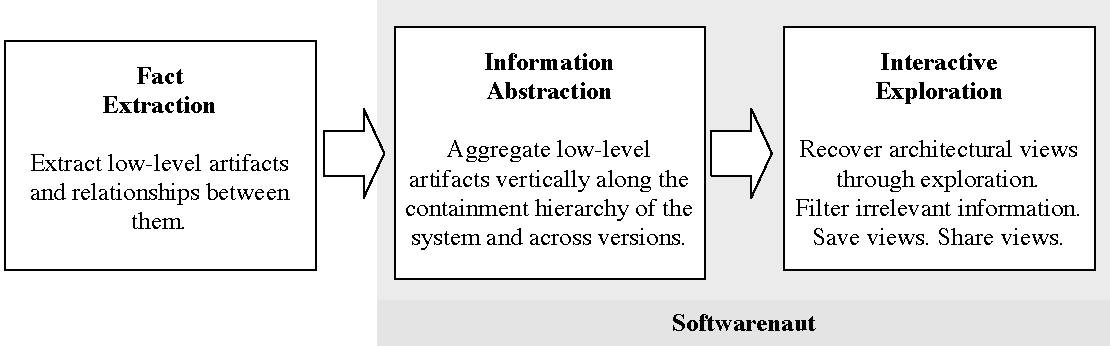
\includegraphics[width=\linewidth]{SnautWorkflow}
\caption{Softwarenaut addresses the last two phases of an {\em extract-abstract-view} process}
\flabel{flow}
\end{center}
\end{figure}

The article continues by detailing the second and third steps, the first one being discussed later in the section on architectural concerns regarding the tool.

%%%%%%%%%%%%%%%%%%%%%%%%%%%%%%%%%%%%%
\section {Information Abstraction} \label{sec:org}
%%%%%%%%%%%%%%%%%%%%%%%%%%%%%%%%%%%%%

Aggregating horizontal relationships between software artifacts along the containment relationships is the fundamental technique that enables abstraction in Softwarenaut. 
\on{! (I wish I knew what that meant)}

\fref{dep-agg} exemplifies the aggregation of low-level relationships between methods and classes along the containment hierarchy of a Java system. The case study is ArgoUML\footnote{Throughout this article we will continue using ArgoUML as a case study. When we do not specify otherwise we refer to version 0.24.} and the figure focuses on the relationships between four classes from three different packages: \cd{uml}, \cd{uml.kernel}, \cd{uml.ui}, and \cd{persistence}. All these packages contain many classes but the visualized entities are sufficient for illustration purposes. 

\begin{figure}[ht]
\begin{center}
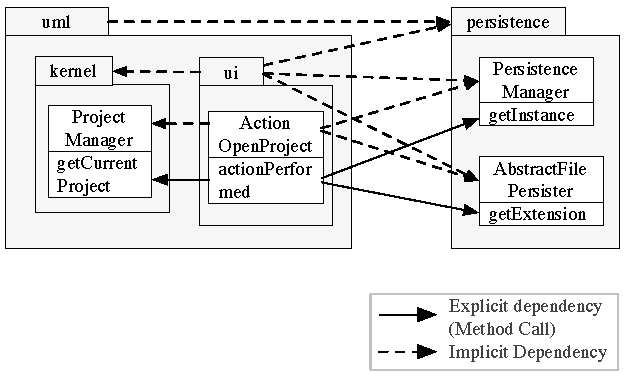
\includegraphics[width=0.75\linewidth]{DependencyAggregation}
\caption{The aggregation of explicit dependencies into implicit ones along the containment hierarchy of methods, classes, and packages in several classes from the ArgoUML case study.}
\flabel{dep-agg}
\end{center}
\end{figure}
 
The figure contains three method calls that can be obtained through static analysis of the system: the method calls between \cd{actionPerformed} and respectively \cd{getCurrentProject}, \cd{getInstance}, and \cd{getExtension}. These explicit relationships propagate as implicit relationships vertically along the containment relationships that exist between methods, classes and packages. Some of the implicit relationships that can thus be derived are the dependencies between the \cd{ui} package and the \cd{PersistenceManager} class as well as the dependency between the \cd{uml} package and the \cd{persistence} package. 


% The figure contains for example the following two explicit low-level dependencies: the method calls between \cod{mX} and respectively \cod{mY} and \cod{mZ}. These explicit dependencies propagate as implicit relationships vertically along the containment relationships (\eg \cod{mX $\rightarrow$ CA2 $\rightarrow$ A2  $\rightarrow$A}, where $\rightarrow$ represents containment relationships). The highest level implicit relationship is the one between A and B. 
% \on{Since it's a foobar example, I have no idea what this implicit relationship is, or whether it makes any sense!}

Aggregating explicit relationships across the hierarchy has a worst case order of complexity of $O(n^2)$ \cite{buchsbaum-hierarchicalgraphs}. Even if in real systems there are never relationships between all the leaves of the tree, so the worst case scenario is never encountered, it is common that for non-trivial systems, the on-the-fly computation of the dependencies can make interactive analysis sluggish. To enable interactivity on large systems it is efficient to pre-compute the dependencies between the nodes in the hierarchy \cite{buchsbaum-hierarchicalgraphs}.
%\on{Nonsense! $O(n^2)$ in theory does not imply $O(n^2)$ in practice!  (The worst-case probably occurs when everything is related to everything else, which is not the case in well-designed software!) You must justify this claim.}



\begin{figure}[ht]
\begin{center}
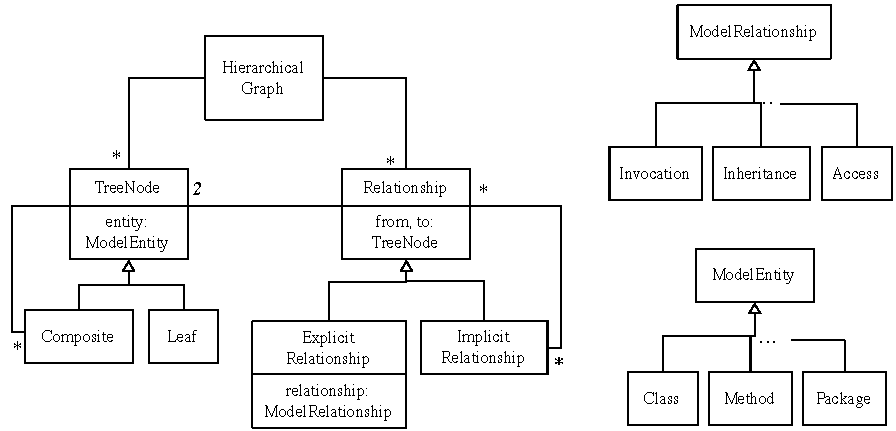
\includegraphics[width=\linewidth]{HigraphModel}
\caption{The {\em hierarchical graph} model in Softwarenaut.
%\on{why do you emphasize "implemented"?}
}
\flabel{hmodel}
\end{center}
\end{figure}

The data structure that Softwarenaut uses to keep track of the pre-computed dependencies in a software system is a {\em hierarchical graph}. The data structure is central to the architecture of the system itself. \fref{hmodel} presents a class diagram of the classes that implement the concept. The figure shows that a hierarchical graph contains two types of entities: 

\begin{description}

\item {\bf Tree Nodes.} These are the wrappers of ModelEntities --- artifacts in a software system that can be organized hierarchically in a containment tree. The diagram shows that the tree is implemented using a Composite design pattern. The objects that the leaves wrap depend on the type of analysis and available data (in some cases they are classes, and in some others they are methods and instance variables). The composite entities are higher-level entities which are either declared in the programming language (such as namespaces and packages) or are obtained as a result of analysis (such as clusters resulting from the hierarchical clustering of the leaves).

\item {\bf Relationships.} There are two types of relationships: {\em explicit} and {\em implicit}.

Explicit Relationships are extracted using both static and dynamic analysis. They often exist between the leaves of the tree (\eg invocations between methods) but not necessarily so (\eg the inheritance relations between classes in a tree which contains both methods and classes). Explicit Relationships wrap actual relationships that are part of the model and which are subclasses of Model Relationship.

Implicit Relationships are derived from the explicit relationships by aggregating them along the containment tree. 

\end{description}

The static analysis of object-oriented system has limitations. One of them is that some dependencies cannot be unequivocally resolved. In the presence of a method that is defined in a base class and overridden in the subclasses it is impossible to know by static analysis to which of the classes a method call will be directed. The decision will be taken by the model extractor. Whatever the decision, the relationships that are extracted by the extractor will be modeled in the hierarchical graph with explicit relationships.

%%%%%%%%%%%%%%%%%%%%%%%%%%%%%%%%%%%%%
%%%%%%%%%%%%%%%%%%%%%%%%%%%%%%%%%%%%%
\newpage
\section {Interactive Exploration} \label {sec:interact}
%%%%%%%%%%%%%%%%%%%%%%%%%%%%%%%%%%%%%
%%%%%%%%%%%%%%%%%%%%%%%%%%%%%%%%%%%%%

\on{This section is really boring because it is presented as a list of disconnected features. It would be more interesting with a running example, showing how all these features are used to explore a specific system.}

The UI of Softwarenaut contains three linked complementary visual perspectives that present information about a system during the exploration. \fref{sos} presents Softwarenaut visualizing an architectural view of itself. 

\begin{figure}[ht]
\begin{center}
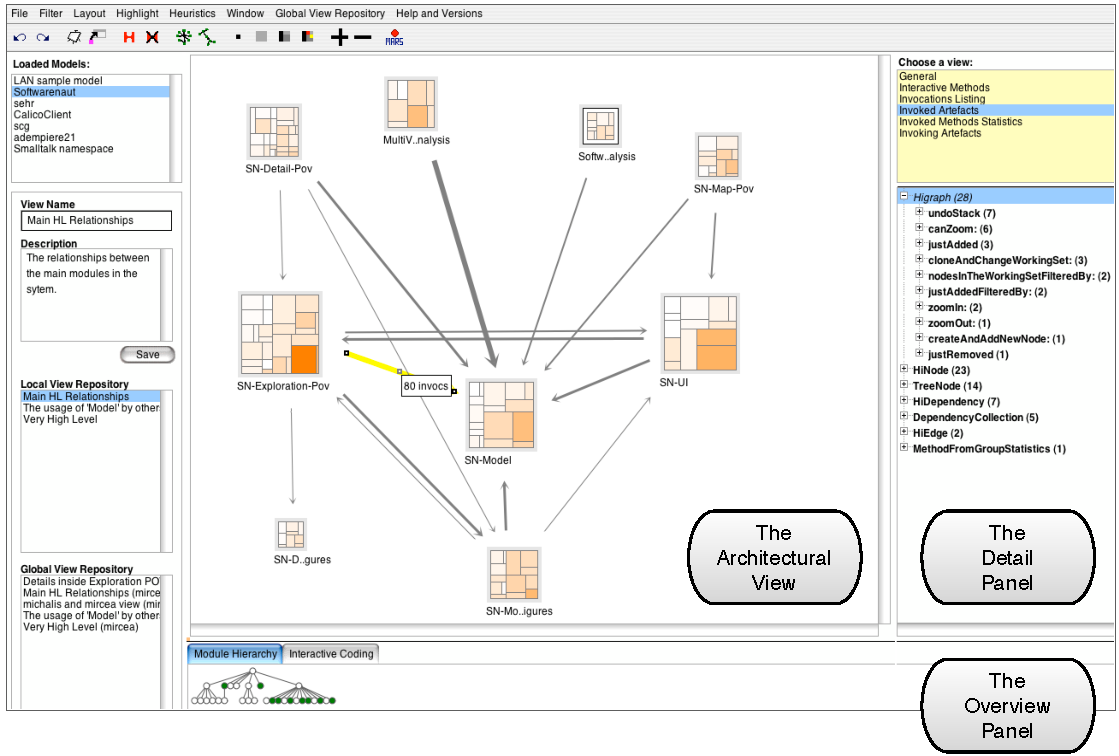
\includegraphics[width=\linewidth]{SnautOnSnaut.pdf}
\caption{Linked views present complementary perspectives on a software system }
\flabel{sos}
\end{center}
\end{figure}

The linked complementary perspectives support the ``overview first, zoom and filter, and details on demand'' architecture of information visualization tools proposed by Shneiderman \cite{shneid-eyes}. 

The three complementary views that the tool supports are the architectural view, the inspector, and the overview panel:

\on{Sometime before here it would be nice to know what Softwarenaut considers an architecture to be. It certainly is not (just) a hierarchy graph.  Architecture is all about constraints and resulting properties.}

\begin{description}

\item The {\em Architectural View} is Softwarenaut's is a graph-based representation of modules and their dependencies. The nodes in the graph represent modules and the edges represent the dependencies between the modules as extracted from the software system. Each dependency edge is an aggregation of low-level dependencies between the two associated modules. 

The tool enables the visualization of a graph at various degrees of visual sophistication. \fref{sofistication} shows three levels of visual detail\footnote{The tool implements also other levels of visual detail. \sref{extensible} presents the way one can extend the tool with new representations for modules.}: (a) the leftmost diagram presents a dependency graph as simple nodes and edges; (b) the middle presents a polymetric view \cite{lanza-pv} in which the width of a dependency is proportional to the number of abstracted explicit relationships, and the size of a module is proportional to its size; (c) the rightmost diagram presents a modified treemap layout which shows all the contained submodules and classes inside a module. 

\begin{figure}[h]
\begin{center}
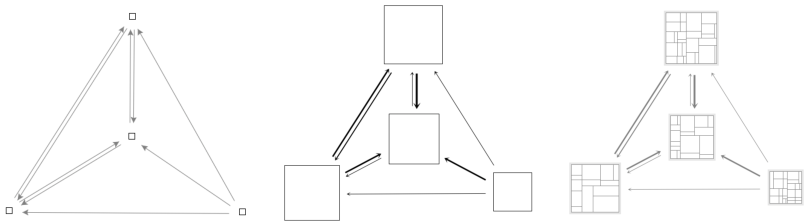
\includegraphics[width=1.04\linewidth]{images/sofistication}
\caption{The tool visualizes a graph with different degrees of sophistication. Left: simple nodes and edges; Middle: polymetric view; Right: a modified treemap view}

\flabel{sofistication}
\end{center}
\end{figure}

\item The {\em Inspector} panel presents details for an entity selected in the Exploration panel. The goal is to supplement details of the element selected in the exploration panel. The detail panel implements the ``details-on-demand'' part of Shneiderman's visualization mantra \cite{shneid-eyes}.
\on{dunno what that is}

\item The {\em Overview hierarchy} presents the entire hierarchy of a system and highlights the modules that are visible in the exploration panel. It presents a vertical slice through a system \cite{wong-thesis}, offering an orientation aid which is critical for successful navigation \cite{storey-awareness}.

\end{description}

In this section we detail the interactive techniques that support the exploration process in Softwarenaut: navigation (\ref{sec:navi}), 
rule-based filtering (\ref{sec:filtering}),
details-on-demand (\ref{sec:dod}). 
%, and visual querying (\ref{sec:vq}).

%%%%%%%%%%%%%%%%%%%%%%%%%%%%%%%%%%%%%
\subsection{Navigation} \slab{navi}
%%%%%%%%%%%%%%%%%%%%%%%%%%%%%%%%%%%%%

The dominant exploration mechanism of Softwarenaut is navigation along the vertical decomposition of the system. One starts with a very high-level abstracted view of a system and continuously refines it by using exploration operations \cite{robertson-conetrees}. At any given moment the set of visible nodes in the exploration view with which the user interacts constitutes the working set (WS). Initially the working set contains very few high-level nodes. As the user explores the system he transforms the working set by performing exploration operations on it and thus changes the contents of the view in the exploration view.

\begin{figure}[ht]
\begin{center}
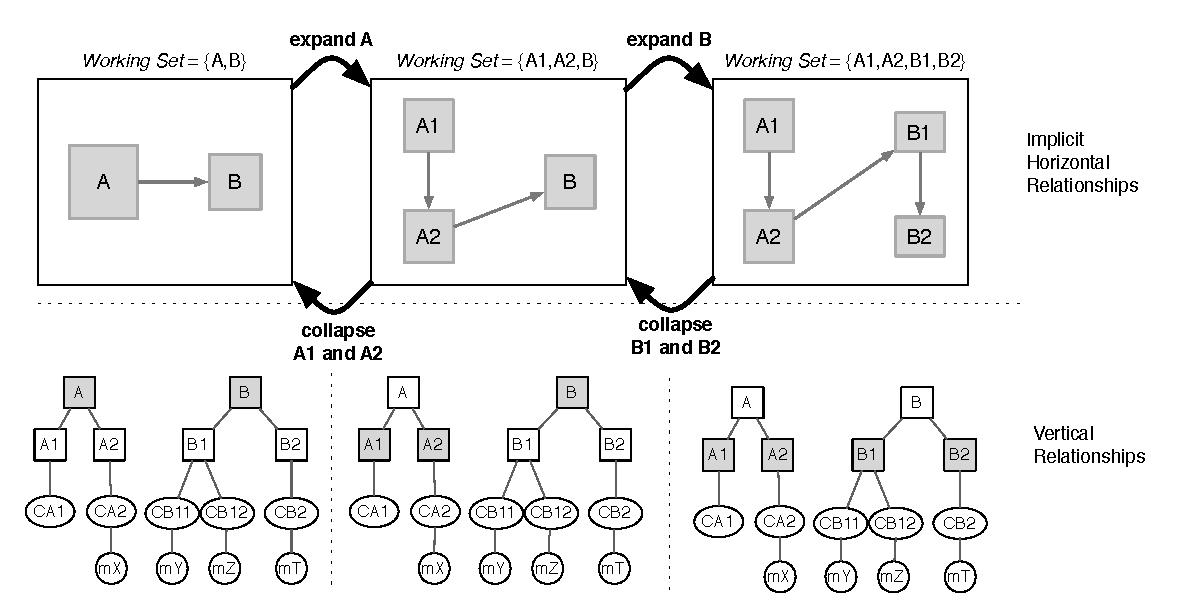
\includegraphics[width=\linewidth]{SnautSequence}
\caption{The expand and collapse complementary operations that \chg{allow}{enable} vertical navigation in the hierarchical graph}
\label{}
\end{center}
\end{figure}

The exploration operations supported by Softwarenaut are:

\begin{description}

\item {\em Expand}. The expand operation applied to a node of the hierarchical graph in the working set replaces the node in the working set with nodes that represent its children. 

%We define the expand operation as follows: 
%
%$ Expand_{N,HG} (WS) = WS - N + Children (N, HG)$, 
%
%where $Children(N,HG)$ is a function which returns the children of node $N$ in hierarchical graph $HG$ and ``+'' and ``-'' represent respectively set union and set subtraction.
%
\item {\em Collapse}. The collapse operation applied to a module in a working set removes the module and all its siblings from the view and replaces them with their parent module. 

%We define the collapse operation as follows:
%
%$ Collapse_{N,HG} (WS) = WS - N - Siblings (N, HG) + Parent (N, HG)$
%
%where $Siblings(N, HG)$ is a function which returns the nodes that have the same parent with $N$ in the hierarchical graph denoted with $HG$, and $parent(N,HG)$ is a function which returns the parent of node $N$ in hierarchical graph $HG$. 
%
\item {\em Remove}. The remove operation applied to a node removes that node from the working set. 

%We define the filter operation as follows:
%
%$ Filter_{N,HG} (WS) = WS - N$
%

\item {\em Group}. The group operation applied to several modules in a working set removes the modules from the set and adds instead a unique new node representing the entire group. 

\item {\em Focus On}. Applied to a node, this operation removes all the nodes and relationships that are not related to a given node from the view and reorganizes the rest of the elements in the view around the node that is under focus.

\item {\em Zoom In}. This operation removes all the other nodes from the view and zooms in into the subject node. It is different than the {\em Expand} ans is useful when expanding the node would bring too much detail into the view. It is in fact equivalent with a {\em Filter} of all the unrelated nodes and then an {\em Expand}.

%We define the group operation as follows: 
%
%$ Group_{N_{i},HG} = WS - N_i + NewGroupNode $
%
%where $N_i$ is the set of nodes the user wants to group.
%
\end{description}

As the user refines the view, and climbs down the hierarchy of the system, he brings more and more elements into the view. He can use the Filter and Group operations on explicit sets of nodes to decrease the number of nodes displayed on screen and therefore cope with the complexity of large graphs. One type of module that benefits the user when filtered out is {\em omnipresent modules} which contribute little to the understanding of the architecture of the system, and heavily clutter the view \cite{mitchell-bunch}.

%%%%%%%%%%%%%%%%%%%%%%%%%%%%%%%%%%%%%
%\subsection {History Operations} 
%%%%%%%%%%%%%%%%%%%%%%%%%%%%%%%%%%%%%

\paragraph {History Operations} An important requirement for information exploration tools is keeping track of the interaction and providing undo/redo operations \cite{shneid-eyes}. Few architecture recovery tools implement this feature. We have discovered this requirement while testing an earlier version of the tool with users (see \sref{usability} for more). In its latest version Softwarenaut implements undo/redo operations.


%%%%%%%%%%%%%%%%%%%%%%%%%%%%%%%%%%%%%
\subsection {Filtering} \slab{filtering}
%%%%%%%%%%%%%%%%%%%%%%%%%%%%%%%%%%%%%

In the previous section we have introduced the {\em Remove} operation which works on explicit sets of nodes. Most software architecture recovery tools offer such a filtering operation \cite{aracic-filtering}. 
Softwarenaut implements two main categories of advanced {\em rule-based filters} for nodes and edges. 
%Softwarenaut supports two main types of filters: 

\begin{enumerate}

\item {\em Low-level filters} act on the hierarchical graph itself. They remove from the hierarchical graph the elements that match a given condition, \eg all the invocation relationships that go to polymorphic classes.

\item {\em High-level filters} act on the high-level elements and relationships between them in the working set, \eg hiding all the high-level dependencies that abstract only a few low-level dependencies.

\end{enumerate}

During exploration, the user needs mostly the high-level filters. There are three types of filters that apply to both artifacts and relationships: 

\begin{description}
\item {\em Metric-based filters} for entities and relationships are defined with respect to the metrics computed for artifacts. For example filtering out {\em the weak dependencies} or {\em the small modules}\footnote{These are threshold-based high-pass filters} in a view

\item {\em Type-based filters} for entities and relationships are defined with respect to the type of the artifacts. For example showing {\em only inheritance relationships} or hiding {\em all the classes} from a view.

\item {\em Evolutionary filters} are defined based on the historical evolution of a module or an inter-module relationship in the system\footnote{Evolution-based filters require models of multiple versions of a system loaded}. For example showing only the {\em relationships that existed in all the versions of a system}, hiding all the {\em unstable relationships} \cite{lungu-relevo}, or displaying only the modules that were introduced in the last version of the system.
\end{description}

\begin{figure}[ht]
\begin{center}
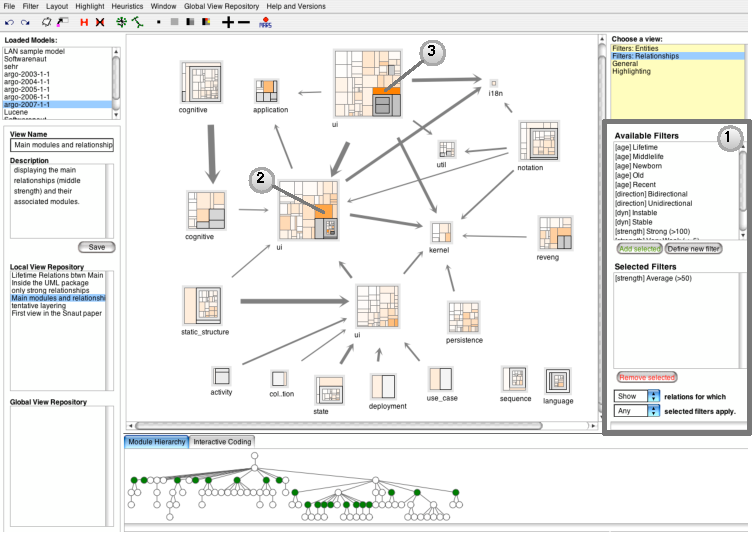
\includegraphics[width=0.95\linewidth]{SnautFilteringPanel}
\caption{The UI for applying relationship filters in Softwarenaut}
\flabel{filpan}
\end{center}
\end{figure}


Softwarenaut also implements filters that work only for relationships. One such example is {\em Directional filters} which are defined based on the direction of the relationship between two modules. For example, filtering out the unidirectional relationships from an architectural view is useful for highlighting the modules that have mutual dependencies between themselves. 
\on{You keep talking about "architecture", but all I see is structure and dependencies. That's not what architecture is all about!}

\fref{filpan} presents the relation filtering panel as implemented in Softwarenaut. Several filters can be combined to obtain more powerful ones with either the ``and'' or the ``or'' operator. The elements that match the filter can be either ``shown'' or ``hidden''. The user can define new filters by writing simple scripts in Smalltalk. \del{The system is fully reflective, and} \on{why is that relevant here?} as soon as a new filter is defined, it will immediately appear in the list of available filters.


\subsection {Highlighting}
Highlighting is related to filtering only in that it does not remove the elements from the view but instead it emphasizes them. One can highlight based on pattern matching in the names of the entities (\eg all the classes that nave ``Test'' in their name) or based on structural properties of the code (\eg all the classes that define the Main method). 

One special type of highlighting can be used for when the modules are represented with a modified treemap view. In that case one can see all the classes in the system in one view and map various metrics that are available for those classes on their color. In \fref{sos} the color intensity of a class is proportional to the FANOUT of that class. With such a view one can discover the hotspots of the system. % -- the number of outgoing calls from that class to other classes in the system.

%%%%%%%%%%%%%%%%%%%%%%%%%%%%%%%%%%%%%
\subsection {Details-on-Demand} \slab{dod}
%%%%%%%%%%%%%%%%%%%%%%%%%%%%%%%%%%%%%

The elements of every architectural view in Softwarenaut are nodes that represent modules and edges that represent relationships between them. For the user to be confident that he {\em understands} such a view he needs to understand the role of every node and the meaning of every edge. Metaphorically, if the view were a phrase, the nodes would be the nouns and the edges would be the verbs. One can understand the message only when he has understood all the nouns and the verbs.

The Inspector panel of Softwarenaut is one of the ways in which one can understand the individual nodes and edges in an architectural view; it presents different views depending on the selected element in the exploration view. 

\on{This is really boring.  It is really just a description of a tool. I am not getting any insight into why any of this is interesting or essential for architectural recovery.}

%%%%%%%%%%%%%%%%%%%%%%%%%%%%%%%%%%%%%
\subsubsection {Inspectors for Modules}
%%%%%%%%%%%%%%%%%%%%%%%%%%%%%%%%%%%%%

% The detail views for modules present various details of a module under focus. Softwarenaut provides a variated set of detail views for nodes that allow understanding the module under focus. 
Understanding and being able to inspect individual modules is part of understanding an architectural view. Softwarenaut provides a series of predefined inspectors for modules. \fref{moduledetails} presents two example views: 

\begin{itemize}

\item The {\em Class List} inspector lists all the classes contained in a module and its submodules together. For these classes the user can select various software metrics. The left figure in \fref{moduledetails} presents the classes in the {\em persistence} module from ArgoUML. The largest class in the system is the class responsible with serializing the UML diagram to disk.

\begin{figure}[h]
\begin{center}
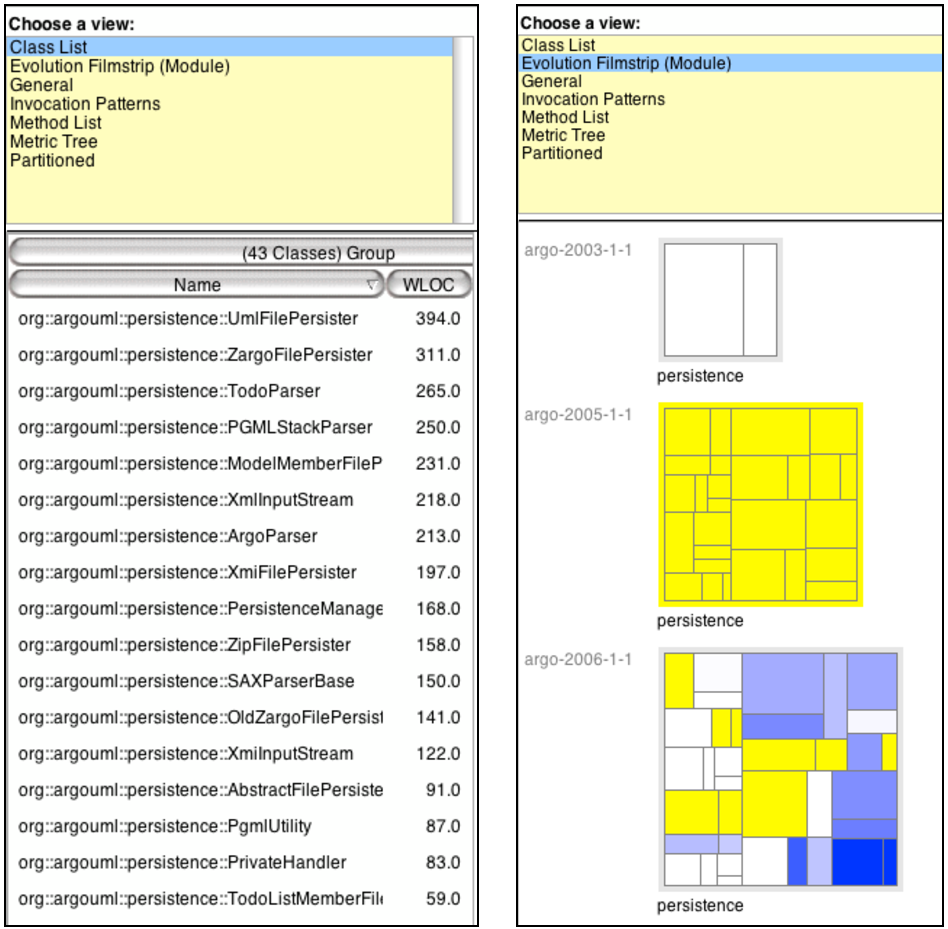
\includegraphics[width=0.75\linewidth]{images/ModuleDetails}
\caption{Two Inspectors: The Class List (left) and the Module Evolution Filmstrip (right) present two complementary aspects of the {\em persistence} module from ArgoUML} 
\flabel{moduledetails}
\end{center}
\end{figure}

\item The {\em Module Evolution Filmstrip} presents the evolution of a given module when multiple versions of the system are loaded. 

The right view in \fref{moduledetails} presents an example. The versions of the module are presented chronologically from top to bottom. In each version evolutionary aspects are highlighted: the classes that are new in that version of the module with respect to the previous one are highlighted with yellow; the classes that are modified with blue and the intensity of the color is proportional to the amount of changes -- the more a class has changed with respect to its previous version, the darker its shade of blue. 

\on{what is the layout strategy? what does the diagram show me? how can I related diagrams in the film strip?}

In \fref{moduledetails} one can see that where the only two classes that existed in the module in the first analyzed version disappear in the second. By inspecting the names of the classes one observes that two classes responsible to interfacing with the database (DBReader and DBWriter) are replaced with classes responsible with writing on the disk.
\end{itemize}
%%%%%%%%%%%%%%%%%%%%%%%%%%%%%%%%%%%%%
\subsubsection {Inspectors for Relationships}
%%%%%%%%%%%%%%%%%%%%%%%%%%%%%%%%%%%%%

Understanding the relationships is critical for understanding an architectural view. Softwarenaut provides a broad and extensible set of inspectors for relationships. They cover both structural and evolutionary aspects \cite{lungu-cutedge, lungu-relevo} of the relationships. \fref{detail-views} and \fref{evostrip} present two types of relationships inspectors: 

\begin{figure}[h]
\begin{center}
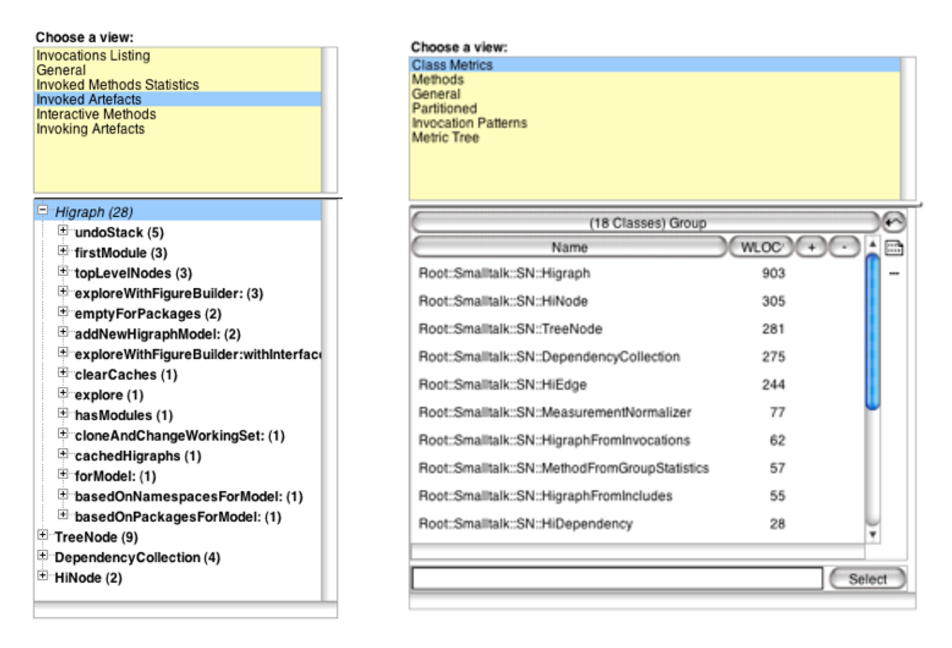
\includegraphics[width=0.5\linewidth]{DetailsForEdgesAndNodes}
\caption{The Invoked Artifacts inspector presents information about the classes that are invoked in a relationship} 
\flabel{detail-views}
\end{center}
\end{figure}


\begin{description}

\item The {\em Invoked Artefacts} view lists all the artefacts invoked by the selected high-level dependency. \fref{detail-views} presents such a view for the dependency between one other module to the {\em cognitive} module in ArgoUML. The tree has on its first level the invoked classes, on the second level invoked methods, and on the third level call sites. The user can navigate to any of the presented code artifacts from this view.

\item The {\em Relationship Evolution Filmstrip} view presents the evolution of the given relationship in all the versions of the system which are available for analysis. \fref{evostrip} presents such a view. The two modules and the associated relationship are represented in every analyzed version with metrics providing information about the dynamics of the relationship. Section \ref{sec:evol} presents more details about the Evolution Filmstrip while discussing evolutionary aspects of the tool.

\end{description}


%\subsection {Visual Querying}


%%%%%%%%%%%%%%%%%%%%%%%%%%%%%%%%%%%%%%%%%%%%%%%%%%%%%%%%%%%%%%%
\section {Evolutionary Analysis} \slab{evol}
%%%%%%%%%%%%%%%%%%%%%%%%%%%%%%%%%%%%%%%%%%%%%%%%%%%%%%%%%%%%%%%

\on{It seems to me that the paper should start with this section.}

Softwarenaut can take evolutionary information into account to provide advanced inspectors and historical filters.


To support multi-version analysis Softwarenaut requires that models of multiple versions of the system under analysis be available. \fref{fig:mva} shows that a system history in Softwarenaut is composed of a list of hierarchical graphs, one for each analyzed version. This approach is conceptually the same as the one of G{\^i}rba \cite{girba-thesis}. One limitation of such an approach is that the number of versions that can be analyzed cannot be too large. As a result one needs a strategy for selecting the versions that compose the history.

To \ugh{\del{allow monitoring}} \on{why "allow"?} \ins{monitor} the evolution of the individual elements through multiple versions one needs to link the corresponding elements in the different versions. Although more complicated approaches are available, in our case we perform a name-based matching of the entities.

\begin{figure}[ht]
\begin{center}
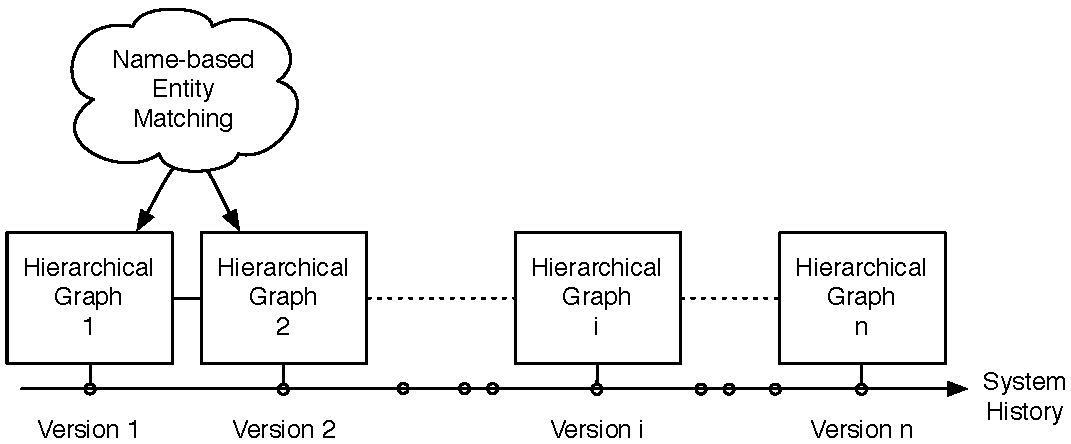
\includegraphics[width=\linewidth]{images/MultiVersionAnalysis}
\caption{In multi-version analysis each version considered has a corresponding hierarchical graph}
\flabel{fig:mva}
\end{center}
\end{figure}

In the following section we show examples of inspectors and filters that take advantage of the available multi-version analysis. 


%%%%%%%%%%%%%%%%%%%%%%%%%%%%%%%%%%%%%
\subsection {Inspectors for Evolutionary Information}
%%%%%%%%%%%%%%%%%%%%%%%%%%%%%%%%%%%%%


One of the applications of multi-version analysis is the {\em Relationship Evolution Filmstrip} \cite{lungu-relevo}. The Filmstrip is an inspector which presents the evolution of a given relationship between two modules over the time. %The view can be useful for understanding a relationship based on its history.

\begin{figure}[ht!]
\begin{center}
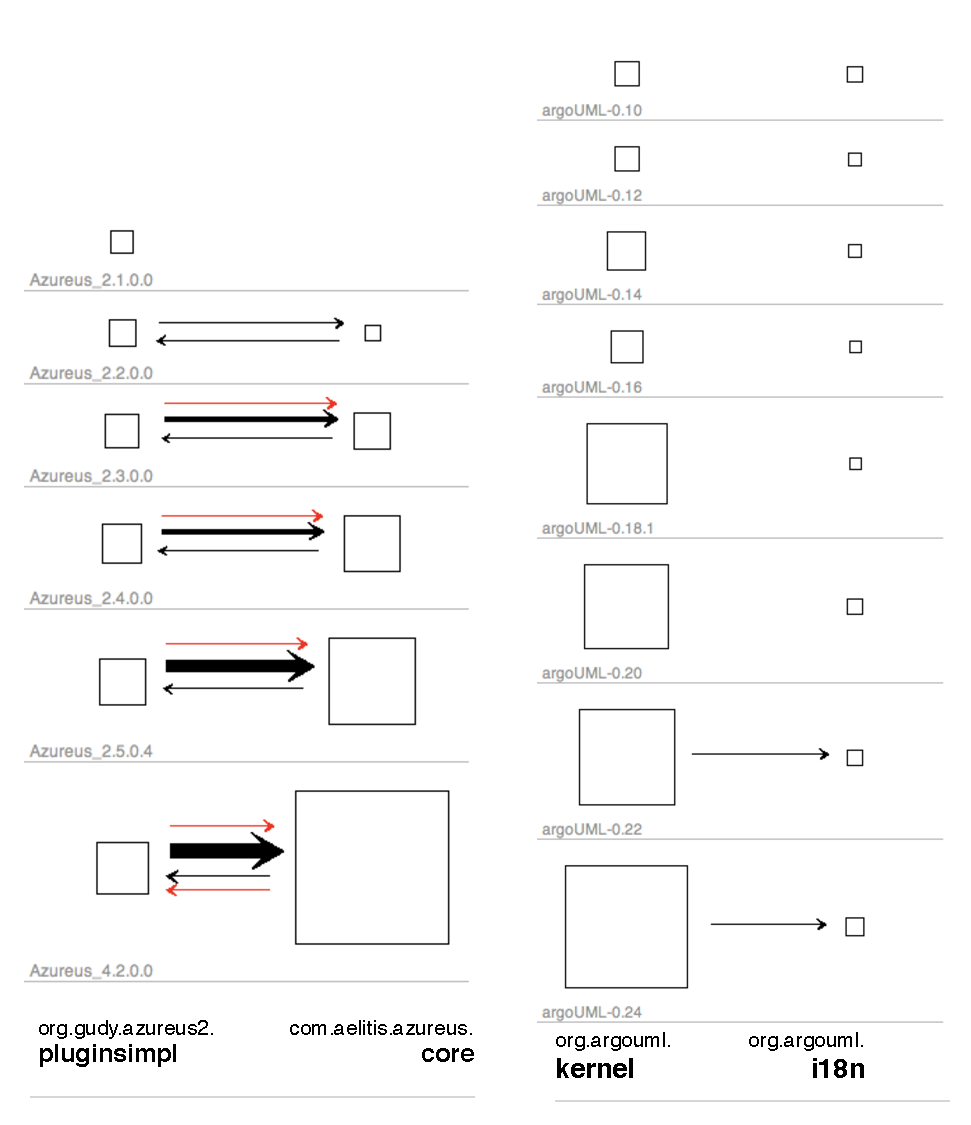
\includegraphics[width=0.8\linewidth]{images/Filmstrip}
\caption{The Relationship Evolution Filmstrip presents the evolution of a given relationship through the multiple versions of the system available for analysis}
\flabel{evostrip}
\end{center}
\end{figure}

\fref{evostrip} presents two examples of relationship evolution filmstrips from Azureus and ArgoUML. In the film strip, the arrows between the modules represent implicit dependencies of different types (the invocation dependencies are represented in black and the inheritance dependencies are represented in red). The width of the dependency arrows is proportional to the number of low-level dependencies abstracted in the corresponding implicit dependency \cite{lungu-relevo}. The representation of the width of the dependencies provides insight into the quantitative dynamics of the inter-module relationship.

In the first case the figure shows that the relationships between the two modules evolved heavily during the evolution. In the second case we see that the relationship is recent and weak: it shows that the kernel depends on the internationalization ({\em i18n}) module. 

%%%%%%%%%%%%%%%%%%%%%%%%%%%%%%%%%%%%%
\subsection {Evolutionary Filters}
%%%%%%%%%%%%%%%%%%%%%%%%%%%%%%%%%%%%%

Filters for relationships and modules are a powerful mechanism for coping with the large graphs that some systems entail. They \chg{allow displaying}{display} only those elements in an architectural view that are important for a given task and thus focus the analysis. Evolutionary filters for both relationships and entities can be classified in two main categories:

\begin{description}
\item {\em Age-based} filters take into account the number of versions in which the relationships or modules existed in the system. {\em Lifetime relationships} have existed in all the versions of the system, {\em Newborn relationship} have appeared only in the last analyzed version \cite{lungu-relevo}, {\em Historical modules} have existed since the first analyzed versions of the system.
\item {\em Dynamics-based} filters take into account the dynamics of the relationships and modules across versions. {\em Stable relationships} do not change much during the evolution of the system, {\em Instable relationships} changed much during the history of the system.
\end{description}

Evolutionary filters assume that not all the entities are equally relevant for the task at hand. Different types of evolutionary filters support different goals of analysis. Two such goals and the corresponding filters are:

\begin{enumerate}

\item {\em Architecture Recovery.} When recovering the architecture of a system one needs to discover first the main components of the system. A filter like {\em lifetime relationships} is relevant since the relationships that existed in the system since the first versions are more likely to be part of the architectural backbone of the system. %TODO Reference.

\item {\em Quality Assessment.} When assessing the quality of an architecture the goal is to find the problems, the irregularities. In this context filters like {\em newborn relationships} are of use since they \chg{allow focussing}{focus} on new relationships that were were not validated by time which might be the result of changes performed by new developers that are unaware of the architecture of the system. %Reference

\end{enumerate}

\fref{lvr} presents two views on the same modules that are also present in \fref{filpan} but with age-based filters activated. The left side presents only the {\em lifetime relationships}: 21 relationships that existed between the displayed modules in all the versions of the system. The right side presents only the {\em newborn relationships}: 36 relationships introduced in the system in the latest version. 

The usefulness of the filters is hinted by the fact that in both the views, the number of relationships is very low compared with the total number of relationships that are present in the last version of the system; ergo, both types of filters function as powerful information reducers.

\begin{figure}
\begin{center}
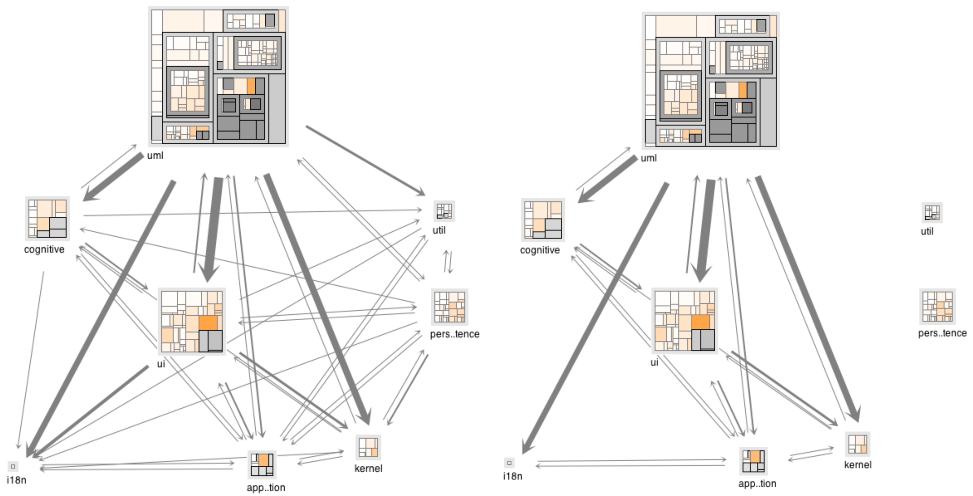
\includegraphics[width=\linewidth]{Architecture-LifetimeVsRecent}
\caption{The left part of the figure shows the {\em lifetime relationships} while the right part of the figure presents the {\em newborn relationships} in the Azureus case study}
\flabel{lvr}
\end{center}
\end{figure}

%%%%%%%%%%%%%%%%%%%%%%%%%%%%%%%%%%%%%
%%%%%%%%%%%%%%%%%%%%%%%%%%%%%%%%%%%%%
\section {Collaboration Through First-Class Views} \slab{views}
%%%%%%%%%%%%%%%%%%%%%%%%%%%%%%%%%%%%%
%%%%%%%%%%%%%%%%%%%%%%%%%%%%%%%%%%%%%

Traditionally software analysis tools were designed with a {\em analysis-in-one-sitting} attitude  in mind. One was supposed to start the analysis, arrive at some results, and then conclude the analysis. In Softwarenaut we want to \chg{allow}{enable} the interruption and continuation of the analysis, and the reuse of the results of the analysis between sessions. Moreover, traditional software analysis never reuses the information that one user has gained about a certain version of the system. This is \chg{wrong}{unfortunate} since once published a version never changes and therefore the results of one analysis can \chg{inform}{contribute to} further analyses. In Softwarenaut these two problems are addressed with the help of {\em first-class views} and the concept of a {\em Global View Repository}, a mechanism for publishing and discovering existing views.

%%%%%%%%%%%%%%%%%%%%%%%%%%%%%%%%%%%%%
\subsection {First-Class Views}
%%%%%%%%%%%%%%%%%%%%%%%%%%%%%%%%%%%%%

The designers of a system use multiple diagrams for the specification of the architecture of a system. In the same way, during architecture recovery they need to recover multiple views to capture various aspects of the structure of the system. 

Views are first-class entities in Softwarenaut: one can save and restore any view during the exploration. During an exploration session, each time the analyst encounters a view which presents a relevant perspective on the system he can save it for later reference. The result of a Softwarenaut analysis is therefore a {\em set of architectural views}.

The view persistence mechanism can be used also as a way of conquering the complexity of top-down exploration. When the architectural view under analysis becomes too complex, the user can save it and then explore different sub-parts of it. This is addressed partially in other tools by the use of semantic zooming techniques \cite{storey-shrimp}. 

In Softwarenaut a {\em view} is defined by the following information: 

\begin{itemize}
\item a name and description,
\item the name and version of the system under analysis
\item the current working set with the positions of all the nodes in it,
\item the active artifact and relationship filters (both explicit and rule based), 
\item the name of the creator of the view
\end{itemize}

The model of the system is not saved together with the view. We assume that model construction is deterministic and the name and version of the system will suffice for model reconstruction at a later time \footnote{This requires nevertheless a way of uniquely identifying the entities in the view. In our case, for each of the entities in the working set we save the fully scoped name}.

%%%%%%%%%%%%%%%%%%%%%%%%%%%%%%%%%%%%%
\subsection {Sharing and Discovering Architectural Views}
%%%%%%%%%%%%%%%%%%%%%%%%%%%%%%%%%%%%%

Once published, a given version of a system never changes. It makes therefore sense to make public all the analysis results regarding that version, so that when other users analyze the same system they can corroborate results and benefit from the previous insights. In the context of architectural view recovery this means discovering architectural views that others have already defined. 

\begin{figure}[ht]
\begin{center}
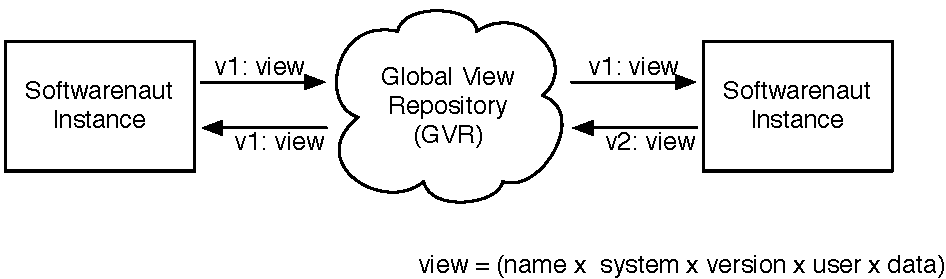
\includegraphics[width=0.7\linewidth]{images/CollaborationConcept}
\caption{Architectural Views are stored in the Global View Repository. This enables collaboration through knowledge sharing and discovery}
\flabel{fig:gvr}
\end{center}
\end{figure}


To support sharing and discovering architectural views we have created the {\em Global Architectural View Repository} (GVR) -- a public repository that indexes architectural views. \fref{fig:gvr} presents the concept behind the GVR through a simplified example. While analyzing system Z, users A and B publish views $v1$ and $v2$\footnote{The $publish(v1,Z)$ notation means publishing to the GVR the view $v1$ for system $Z$}. When later user M analyzes the same system, he can already benefit from the previous knowledge by discovering the views that users A and B have published. 


The architectural views as saved in the GVR can serve as the basis for monitoring the architectural evolution of the system. After the publication of a new version of the system, Softwarenaut can automatically detect the views affected by the new changes, and present a {\em visual diff} on top of the view retrieved from the GVR between the state of the system at the moment the view was created and the latest commit.

\begin{figure}[ht]
\begin{center}
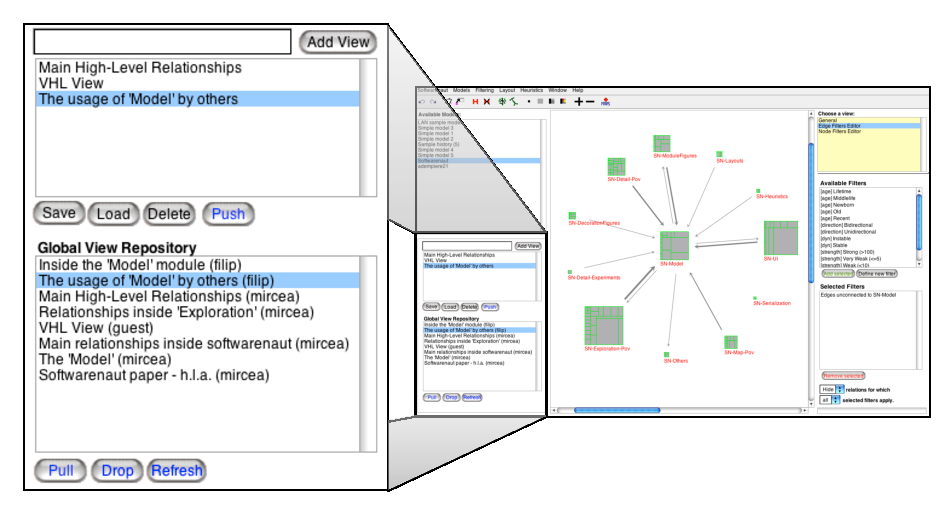
\includegraphics[width=1.05\linewidth]{ViewOperations}
\caption{Views are first-class entities in Softwarenaut. They can be saved, deleted locally, but also published and retrieved from the Global Architectural View Repository.}
\flabel{viops}
\end{center}
\end{figure}

\fref{viops} presents the current state of the UI which is responsible with the interaction with the architectural views in Sofwarenaut: 

\begin{itemize}

\item The top part of the inset presents the locally stored views which the user has in the image. For each of them the user can load it, delete it, or push it to the GVR. In the inset, the buttons which have black text represent operations that can be applied on the local views.

\item The bottom part presents the views which exist for the given system in the GVR. From the global view repository he can pull views in the local repository, or if he is the creator of such a view he can delete it from the global repository too. 

\end{itemize}


%%%%%%%%%%%%%%%%%%%%%%%%%%%%%%%%%%%%%
%%%%%%%%%%%%%%%%%%%%%%%%%%%%%%%%%%%%%
\section {Architectural Considerations Regarding Softwarenaut} \slab{archi}
%%%%%%%%%%%%%%%%%%%%%%%%%%%%%%%%%%%%%
%%%%%%%%%%%%%%%%%%%%%%%%%%%%%%%%%%%%%

\on{strange section heading}

%%%%%%%%%%%%%%%%%%%%%%%%%%%%%%%%%%%%%
\subsection {Fact Extraction and Modelling} \label{sec:facts}
%%%%%%%%%%%%%%%%%%%%%%%%%%%%%%%%%%%%%

At the lowest level, Softwarenaut models a system using the Core of the FAMIX meta-model \cite{tichelaar-thesis}. \on{What's that? Never heard of it ...} \ins{FAMIX is ...} Given that the meta-model is language independent, Softwarenaut can analyze any system written in an object-oriented language. This requires fact extractors that analyze the source code and build the intermediary model. For this we use various third-party tools like McC \cite{pepi-mcc} or inFusion\footnote{See \url{http://www.intooitus.com/inFusion}, verified Jan 25 2011.}.  

FAMIX represents both artifacts and relationships as first-class entities. The main artifacts are namespaces, packages, classes, attributes, methods, fields. The main relationships between these entities are method invocations, variable accesses, class inheritances, and package include relationships \cite{tichelaar-thesis}.

A class of relationships \chg{which}{that} have a special importance in Softwarenaut are the containment relationships which organize a software system into a vertical hierarchy: classes contain methods, modules contain classes, systems contain modules. This containment mechanism is a \chg{powerful}{conventional} way of coping with the complexity of large software systems.

At an architectural level, different languages provide different mechanisms for the hierarchical organization of the system. C/C++ developers use the directory structure to organize systems hierarchically; Java developers use the package hierarchy; Smalltalk developers use the bundles hierarchy, etc. 
When a hierarchical decomposition is not provided, we can automatically generate one using clustering techniques \cite{koschke-thesis}. We presented elsewhere an experiment in clustering the classes in a system based on language similarity\cite{Lung05a}.

%%%%%%%%%%%%%%%%%%%%%%%%%%%%%%%%%%%%%
\subsection {Integration with the Moose Analysis Platform}
%%%%%%%%%%%%%%%%%%%%%%%%%%%%%%%%%%%%%


Softwarenaut is integrated in the Moose Analysis Platform \cite{nier-story}. Softwarenaut reuses several of the views defined in Moose for its inspectors (\eg the inspectors that show entity metrics). Also, since behind any visual element of Softwarenaut lays a TreeNode object which wraps often a FAMIX entity (\eg FAMIXPackage or FAMIXClass) the user can spawn other Moose analyses by selecting any of the elements of a Softwarenaut architectural view. At the same time, any tool in the Moose platform can spawn a Softwarenaut architectural analysis on any group of entities which have containment relationships and dependencies between themselves.

\subsection {Mechanisms for Tool Extension}
\label{sec:extensible}
%The tool is built with extensibility in mind. 
Many of the features of the tool are loaded at run-time through \ugh{reflexion} \on{use consistent spelling!} so that that all one needs is to know the extension points. Here we give examples of several of the features that are loaded \ugh{reflexively} together with the rules by which they are discovered.

\begin{description}
\item {\em Inspectors for Modules and Dependencies}. In order to provide a new inspector for a module or a relationship one needs to implement a subclass of {\em Inspector} which implements three messages: \cd{canDisplay: anObject}, \cd{tabName} and \cd{display: anObject}. The first message tests whether the inspector can display a certain object, the second gives the name of the view, and the third actually displays the object. \fref{filmstrip-sample} shows the implementation of the first two methods in the Relationship Filmstrip\footnote{The examples are in Smalltalk}.

\begin{figure}[h]
\begin{center}
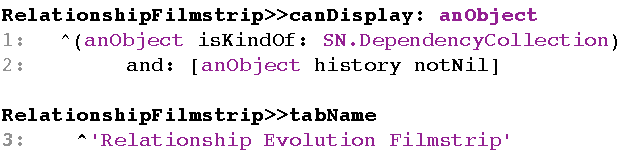
\includegraphics[width=10cm]{images/filmstrip-sample}
\caption{Two methods \chg{allow}{enable} the runtime discovery of inspectors}
\flabel{filmstrip-sample}
\end{center}
\end{figure}

\item {\em Filters for Modules and Dependencies}. In order to provide a new filter one needs to add a new method in the corresponding filter class (\cd{NodeFilter} or \cd{DependencyFilter}) and annotate it with the \cd{filter} annotation. \fref{filter-sample} shows the code for the definition of the {\em newborn} relationships -- these are relationships that have a history of size one (line 5) and their last version is not empty (line 6). Line 1 shows the annotation.

\begin{figure}[h]
\begin{center}
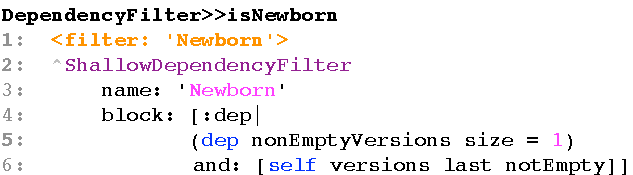
\includegraphics[width=10cm]{images/filter-sample}
\caption{Annotating methods in the Filter classes \chg{allows}{enables} run-time discovery}
\flabel{filter-sample}
\end{center}
\end{figure}


\item {\em Module Representations}. In order to provide a new method for representing a module one needs to subclass the \cd{ModuleFigureBuilder} class and implement the \cd{moduleFigureFor:withBounds:} message in his new class. The method receives the object it is supposed to draw together with the rectangle in which it has to fit the visual representation of the object.

\end{description} 


%%%%%%%%%%%%%%%%%%%%%%%%%%%%%%%%%%%%%
\subsection {Softwarenaut Synergies}
%%%%%%%%%%%%%%%%%%%%%%%%%%%%%%%%%%%%%

One of the tools that benefits from the Global View Repository is the Small Project Observatory (SPO), an ecosystem analysis tool that we have introduced elsewhere \cite{lungu-est}. SPO works at an abstraction level above the architectural level of individual systems: the {\em ecosystem abstraction level} \cite{lungu-thesis}. 

\begin{figure}[ht]
\begin{center}
\includegraphics[width=\linewidth]{SpoArchitectural}
\caption{SPO imports architectural views saved in Softwarenaut}
\label{}
\end{center}
\end{figure}

SPO needs to support navigation between the two abstraction levels to support the understanding of  the ecosystem abstraction level. When navigating from the ecosystem abstraction level down to the architectural level SPO must present architectural views of the individual systems. When they are available, the architectural views of the individual systems are obtained from the Global View Repository. SPO can therefore reuse architectural information generated with Softwarenaut.

One of the limitations of Softwarenaut is the reliance on external fact extractors. This means that finding case-studies was always less than straightforward. To address this, in a collaboration with the researchers at UC Irvine we have integrated the tool with the SourcererDB database \cite{linstead-sourcerer}. Softwarenaut has now a broad range of available case-studies while the database can benefit from the analysis services of Softwarenaut. The integration with the SourcererDB was eased by the service based architecture of Sourcerer and intermediated by the FAMIX meta-model: Sourcerer provides a service which exports FAMIX models of its systems. 


%%%%%%%%%%%%%%%%%%%%%%%%%%%%%%%%%%%%%
%%%%%%%%%%%%%%%%%%%%%%%%%%%%%%%%%%%%%
\section {Tool-Building Considerations} \label {sec:disc}
%%%%%%%%%%%%%%%%%%%%%%%%%%%%%%%%%%%%%
%%%%%%%%%%%%%%%%%%%%%%%%%%%%%%%%%%%%%

In this section we discuss several aspects related to tool-building in research. We touch usability, the integration in the broader research ecosystem, and using the tool as a testbed for research.


\subsection {The Tool as a Vehicle for Research}
Softwarenaut served as the prototype for many of the research ideas we had during the PhD of the first author. We have integrated the tool with others \cite{lungu-clust, lungu-scico, nier-story} and we provided a framework in which master projects can be developed \cite{boeckmann-mars}. %We have also used the tool several times to perform reverse engineering in consulting projects.
The tool was the basis for a number of research papers: 
\begin{itemize}
\item {\em Package Patterns for Architecture Recovery} \cite{lungu-packages}: This article provides a classification of software packages based on their interaction with the rest of the system. We used Softwarenaut to explore multiple systems and discover these patterns.
\item {\em Exploring Inter-Module Relationships in Software Systems} \cite{lungu-relevo}: This article presents a taxonomy of inter-module dependencies in software systems based on their evolution patterns.
\item {\em Interactive Exploration of Semantic Clusters} \cite{lungu-clust}: This article proposes a technique for visualizing dendrograms of software systems using an exploration approach. In order to be able to visualize \ugh{dentrograms} \on{dendograms?} resulting from hierarchical clustering we had to adapt our model.
\item {\em Cutting Edge Visualization in Software} \cite{lungu-cutedge}: This short article argues for the importance of providing detail views that allow one to understand dependencies in software.
\end{itemize}

%\cite{lungu-cutedge, lungu-clust, lungu-packages, lungu-relevo}. 
%For these articles Softwarenaut was the vehicle through which the associated studies could be performed or the ideas could be implemented. The tool served as a testbed for our ideas. %One of the research directions that we use the tool for nowadays is studying how to better support collaborative efforts in architecture recovery.


%In the next section we present a brief discussion on evaluating the tool with students.

\subsection {Studying the Usability of the Tool}
\label{sec:usability}
We have often used Softwarenaut to analyze Softwarenaut itself, and this has determined several re-architecting sessions as well as UI improvements. We also used the tool in the practical part of the Software Evolution master course at the University of Lugano to test its usability and usefulness. 

\begin{table}[b!]
\begin{center}
\begin{tabular}{l p{\linewidth}}
& \footnotesize{Task} \\ \hline
\footnotesize{1} & \footnotesize{Discover one or more architectural views on the system which present modules and their interactions} \\
\footnotesize{2} & \footnotesize {Is there a subset of the modules that you consider to be at the core of the system?} \\
\footnotesize{3} & \footnotesize {Is there a core module in the system? Why? How does it interact with the others?} \\
\footnotesize{4} & \footnotesize {Choose one inter-module dependency in the system and analyze it. What is the reason for its existence?} \\
\footnotesize{5} & \footnotesize {Choose one other module in the system. Analyze its interface.} \\
\footnotesize{6} & \footnotesize {Are there cases in which two modules depend on one another that you would have not expected from the conceptual architecture?} \\
\footnotesize{7} & \footnotesize {Overall what do you think about the structure of the system? Is it well modularized?} \\
\footnotesize{8} & \footnotesize {You want to add support for generating code in a new language. Which module do you change? Which others are impacted? How much time do you need?} \\ \hline
\end{tabular}
\caption{The eight tasks the participants had to solve in two hours.}
\label{tab:questions}
\end{center}
\end{table}

In the second year of using the tool in the Software Evolution course we decided to have an exploratory study to evaluate the usability and usefulness of the tool. We asked the students to analyze a large software system they have never seen before with the help of Softwarenaut and to produce an architectural report. Our main goal in organizing the experiment was to get feedback on the usability of the tool; our second goal was to collect anecdotal evidence on its usefulness for architecture recovery.

Eight users, one PhD and seven master students participated in the experiment. We presented the tool during one hour. Then they had two hours to perform the tasks presented in \tref{questions}. The case study was ArgoUML. We had them work in teams of two and asked them to provide us with a report of their findings. After providing us with the report, they were asked to respond to a questionnaire on the usability of the tool. 


By analyzing their reports we observed several things:

\begin{itemize}
\item In several of the tasks (1--3) each of the teams provided a slightly different perspective on the system. The differences were in the layouts they used, in the filtering they applied. Each one captured a certain aspect of the system. Unfortunately at the time there was no way for them to share the views with each other and discuss them.
\item Some of the tasks were not solved by all the teams (4--5,8). One reason was the insufficient training with the tool, another reason were the usability limitations of the tool at the time of the experiment. %\footnote{We will discuss these limitations later. }
\item For one of the tasks (8) the tool was not sufficient and they had to rely on the online documentation of the analyzed system. 
\item For the questions regarding dependencies (4,8) all the users preferred the tool to reading the code or online documentation.
\end{itemize}

After they submitted their reports we asked the users to fill a questionnaire and evaluate the usability of the tool. 

The first part of the questionnaire contained several assertions. The users had to mark the strength of their agreement with each assertion on a scale from 1 to 5. \tref{postsurvey} presents the assertions together with the average agreement level. Although not statistically relevant the results show that the tool was easy to use, the participants felt confident that the results they provided were reliable.%, and they found the dependency analysis easy to use. 
 There was less agreement on whether the user interface was intuitive and whether ArgoUML was an appropriate case study. We believe that these two last answers were due to the limited time they had at disposition. %to accommodate themselves with the tool and the difficulty of ArgoUML as a case study.

\begin{table}[ht]
\begin{center}
\begin{tabular}{p{8cm} r}
\footnotesize{Assertion} & \footnotesize{Agreement Level (average)} \\ \hline
\footnotesize{The tool was simple to use} & \footnotesize{4}  \\
\footnotesize{The user interface was intuitive} & \footnotesize{3.25} \\
%\footnotesize{It was easy to discover dependencies between modules} & \footnotesize{4.25} \\
\footnotesize{The results generated were reliable} & \footnotesize{4.5} \\
\footnotesize{Was ArgoUML a good choice for a case study?} & \footnotesize{3} \\ \hline
\end{tabular}
\caption{Answers to the questions regarding the tool usability }
\label{tab:postsurvey}
\end{center}
\end{table}

The second part of the questionnaire were open questions. We first asked the participants what were the capabilities of the tool that they found the most useful during their analysis. Two of the teams answered with {\em "all the features we have used"} and {\em "many features, you can do a lot"}. \tref{useful} shows that the others were content with the dependency analysis and the exploration operations.

\begin{table}[ht]
\begin{center}
\begin{tabular}{l l}
\footnotesize {Feature} &\footnotesize{ Supporters} \\
\hline
\footnotesize {Showing dependencies between modules} & \footnotesize{(2 teams)} \\
\footnotesize {The exploration operations} &\footnotesize{(2 teams)} \\
\footnotesize {Filters} &\footnotesize{(1 team)} \\
\footnotesize {Inspectors} &\footnotesize{(1 team)} \\
\hline
\end{tabular}
\caption{The features that the users considered the most useful}
\label{tab:useful}
\end{center}
\end{table}

We finally asked what were the features that they thought were missing from the tool. \tref{missing} shows that the most desired features were smart filters, arbitrary groupings and history operations.

\begin{table}[ht]
\begin{center}
\begin{tabular}{p{0.8\linewidth} r}
\footnotesize {Feature} &\footnotesize{ Requesters} \\
\hline
\footnotesize {User defined filters (all incoming dependencies, all outgoing dependencies, dependencies weaker than...)} &\footnotesize{ (3 teams)} \\
\footnotesize {Arbitrary grouping of items (selected items, classes whose name matches a certain pattern, orphan classes)} &\footnotesize{ (3 teams)} \\
\footnotesize {Undo and Redo operations} &\footnotesize{ (2 teams)} \\
\footnotesize {Selecting edges (multiple edges, all outgoing edges)} &\footnotesize{ (2 teams)} \\
\footnotesize {View persistence} &\footnotesize{ (1 teams)} \\
\hline

\end{tabular}
\caption{The features that the users considered were missing}
\label{tab:missing}
\end{center}
\end{table}

We had used these results to inform our work on future versions of the tool. Many of these features are included in the tool and have been presented in this article while some are still on the backburner. \footnote{One usability problem which, although not on the list of our participants, we are aware of is the fact that when too many nodes are expanded the view becomes to busy to be useful. We have observed that effect depends heavily on the structure of the system that is being analyzed. }


This has been an early exploratory study with few participants and we cannot claim that the results generalize. In the future we plan to organize a controlled experiment to evaluate both the usefulness of the tool for the purpose of architecture recovery as well as its usability.

%%%%%%%%%%%%%%%%%%%%%%%%%%%%%%%%%%%%%
\subsection {Depending on Other Research Prototypes }
%%%%%%%%%%%%%%%%%%%%%%%%%%%%%%%%%%%%%

Depending on other research prototypes and platforms has been a benefit because we had the opportunity of using cutting edge technology and building on the shoulders of giants. In the same time it made our life harder since the tools that we depended on kept moving ``under our feet'' and at times they were not maintained anymore. 

For example during the development of the tool the Moose framework was ported from VisualWorks Smalltalk to Pharo Smalltalk for license reasons. Together with this the FAMIX 2.1 meta-model was replaced with the 3.0 version. This introduces a small compatibility issue between the tools that work in Pharo and VisualWorks. Since until now we did not have the engineering effort required to port all our code to Pharo we remained dependent on the VisualWorks Moose version. 

A totally different problem is when one depends on a web service. There one cannot shield oneself from the changes on the other side. Recently the SourcererDB went through a database upgrade: for some time the Softwarenaut users did not have access to the large pool of case studies.

This might not be a unique experience, but it is a reminder that when building research prototypes that relies on other research prototypes one needs either to shield oneself from changes upstream or to be ready to constantly adapt to the changes. We believe that the best strategy is a combination of both and that the benefits of being part of a research ecosystem outweigh the difficulties.

%%%%%%%%%%%%%%%%%%%%%%%%%%%%%%%%%%%%%
\subsection {Availability and Documentation}
%%%%%%%%%%%%%%%%%%%%%%%%%%%%%%%%%%%%%

Softwarenaut is written in Smalltalk and is released under the open source MIT License. The tool is available online at {\footnotesize \url{http://scg.unibe.ch/softwarenaut/}}. The homepage of the tool provides screencasts, documentation, installation instructions, and directions on how to obtain the source code and to contribute.

The Global Architectural View Repository (GVR) is implemented as a PostgreSQL database which can be publicly accessed by instances of Softwarenaut or other tools. The online documentation provides more informations about ways of accessing the GVR. 

%%%%%%%%%%%%%%%%%%%%%%%%%%%%%%%%%%%%%
\section {Related Work} \label {sec:rel}
%%%%%%%%%%%%%%%%%%%%%%%%%%%%%%%%%%%%%

There is an extended tradition of architecture recovery tools in software engineering research. Pollet \etal have presented a comprehensive overview of the work in architecture recovery in their survey article \cite{pollet-sar}. In this section we take several of the core aspects of Softwarenaut and we discuss how they are similar and how they differ from other state of the art tools.

%%%%%%%%%%%%%%%%%%%%%%%%%%%%%%%%%%%%%
\subsection {Exploration and Navigation} 

The first architectural visualization prototype was Rigi, a programmable reverse engineering environment which emphasizes visualization and interaction \cite{muller-revengenv}. Rigi  visualizes the data as hierarchical typed graphs and provides a Tcl interpreter for manipulating the graph data. The reconstruction process is based on a bottom-up process of grouping  software elements into clusters by manually selecting the nodes and collapsing them. The approach does not scale when analyzing very large systems because the number of low-level artifacts is too large. This is why in Softwarenaut we automatically aggregate low-level relations, and then let the user navigate from the highest abstraction level downwards is the main interaction approach in Softwarenaut. 

One of the projects inspired by Rigi was the SHriMP tool \cite{storey-shrimp} and its Eclipse-based continuation Creole \cite{lintern-creole}. SHriMP and Creole display architectural diagrams using nested graphs. Their user interface embeds source code inside the graph nodes and integrates a hypertext metaphor for following low-level dependencies with animated panning, zooming, and fisheye-view actions for viewing high-level structures. The difference to Creole is that Softwarenaut can also perform evolutionary analysis.


%%%%%%%%%%%%%%%%%%%%%%%%%%%%%%%%%%%%%
\subsection {Evolutionary Analysis}
 
YARN \cite{hindle-yarn} animates the evolution of dependencies between the modules of a system. We represent evolution by building complete models of several system versions (just like CodeCity) while YARN uses an evolutionary model and analyze the information in each commit. The disadvantages of YARN is that watching an animation can be time-consuming and it does not support interactive exploration operations such as filtering. 

CodeCity of Wettel \cite{wettel-icse11} visualizes software systems using a city metaphor and also provides visualizations of the evolution of the systems. The main advantage of our approach over  Wettel's is the fact that we present relationships while he does not. However, one advantage of his work is that his views are always clean while in our case sometimes too many relationships clutter the view.

Pinzger proposed the ArchView approach \cite{pinzger-thesis} which provides visualizations that present the evolution of the modules in a system. His evolution analysis takes into account the annotations from the versioning system repository. However, there is no support for first-class views in ArchView and the dependencies between the modules are only based on logical coupling. 

One of our original contributions is the possibility of filtering information in the view based on its historical properties. One related study is the one of Wierda \etal who recover the architectural decomposition of a system through clustering; they observe that if they use for clustering only those dependencies that were in the system in both the first and the last versions, the decompositions are more precise \cite{wierda-clustering}. This observation supports our idea of considering the lifetime relationships as more relevant for the architecture than the newer relationships. 

%%%%%%%%%%%%%%%%%%%%%%%%%%%%%%%%%%%%%
\subsection {Collaboration} 

Shrimp, the tool of Storey \etal, also allows for saving and restoring views \cite{rayside-flow}. The views are saved inside a ``Filmstrip'' which is persistent. Through the intermediation of the filmstrips the users can restore exploration sessions or even share certain views. This type of information \chg{allows}{enables} people that know about each other to share information by emailing the files. The advantage of the Global View Repository is that it \chg{allows to share information that other users have discovered.}{allows information that other users have discovered to be shared}.

The work of D'Ambros \etal on Churrasco \cite{dambros-churrasco} and the work of Hattori \etal  on Replay \cite{hattori-replay} are related to both the collaboration and evolutionary aspects of our tool. Churrasco supports software evolution modeling, visualization and analysis through a web interface. Through an example scenario they show that Churrasco allows for collaborative software evolution analysis, and they attribute this to the availability on the web of the tool. Replay allows for the chronological replay of changes inside the Eclipse IDE and it supports awareness of team member activity by allowing one to selectively replay the changes of other team members. The information in Replay is much more fine-grained and precise than in our case; it however stays at the lowest level of abstraction while we are interested in architecture. Churrasco presents high-level visualizations but it does not provide dependency information which we consider critical for architectural understanding. 

One project developed with collaboration support as the main goal is the Jazz IDE of IBM \cite{hupfer-jazz}. 
In their case they aim at supporting collaboration and awareness in small informal software development teams during forward engineering. In our case we use the Softwarenaut to support collaboration between engineers during program understanding although architectural views once recovered can be used to support evolutionary awareness during forward engineering: the Jazz dashboard could benefit from integrating architectural views which highlight system evolution.

%%%%%%%%%%%%%%%%%%%%%%%%%%%%%%%%%%%%%%
\section {Conclusions and Future Work} \label {sec:conc}
%%%%%%%%%%%%%%%%%%%%%%%%%%%%%%%%%%%%%%

We presented Softwarenaut, our tool for architecture recovery. Softwarenaut allows the recovery of architectural views of a software system through interactive exploration. It supports the ``overview first, zoom and filter, and details on demand'' principle of information visualization. It provides powerful filtering mechanisms and the capacity of saving and sharing architectural views. The tool was the test-bed for a variety of research projects and is still serving us in our research and consulting practice. 

There are two main research directions in which we would like to bring Softwarenaut beyond architecture recovery:

\begin{description}

\item {\em Reengineering.} One of the tools built on top of Softwarenaut is MARS, an automated architecture refactoring recommender tool \cite{boeckmann-mars}. MARS starts from a given Softwarenaut view and checks whether move operations applied on classes can improve the architecture of the system by increasing coupling and decreasing cohesion. Preliminary results show a good recall but a low precision of the automated refactoring recommendations generated by MARS. We plan to explore more reengineering operations that can be performed on an architectural view.

\item {\em Monitoring Software Evolution.} One of our future projects is exploring ways in which the recovered views can function as a live documentation of an evolving system. The Softwarenaut views are not simple pictures but instead they code relationships between the modules of the system. A view recovered for a given version of the system can function as a reference point for presenting the future evolution of the system. After the publication of a new version of the system, Softwarenaut can automatically detect the views affected by the new changes, and visualize these changes on them.

\end{description}

\paragraph{Acknowledgements} We would like to thank Fabrizio Perin and Niko Schwarz for feedback on earlier drafts of this paper. We would like to acknowledge Joel Ossher who provided the web-service which exports FAMIX models from the SourcererDB database. We would also like to thank the anonymous reviewers for their constructive feedback and the patience they had while trying out Softwarenaut. Lanza acknowledges the financial support of the SNF through project SOSYA (SNF Project No. 132175).

\bibliographystyle{model1-num-names}
\bibliography{scg,mircea}

\end{document}
